\section{Processing of a Single Subject-Verb Dependency in NLMs}
In the classic number agreement task (NA-task), subjects are presented with the beginning of a sentence (aka, `preamble') that contains a long-range subject-verb relation, such as: ``The \textbf{keys} to the \emph{cabinet}\ldots'', and are asked to predict the verb to follow (e.g., ``are''). 
Human subjects make more agreement errors (e.g., continuing the preamble  above with ``is'' instead of ``are'') when the intervening noun (aka, `attractor') has a different grammatical number than the main subject (as in the preamble above, with plural subject ``keys'' and singular attractor ``cabinet'') \citep{Bock:Miller:1991}.
Behavioral measures collected during agreement tasks, such as error rates, vary as a function of the syntactic environment of the long-range dependency. This has provided rich data to test hypotheses regarding online syntactic processing in humans \citep[e.g., ][]{franck2002subject, franck2006agreement, franck2007syntactic}.

Starting with the influential work of \citet{Linzen:etal:2016}, a growing
literature \citep[e.g.,][]{Gulordava:etal:2018, Bernardy:Lappin:2017,
  Giulianelli:etal:2018, Kuncoro:etal:2018a,Linzen:Leonard:2018,jumelet2019analysing} has
tested NLMs on the NA-task at the behavioural level, showing that these models have performance and error patterns partially resembling those of humans.
Recently, \citet{lakretz2019emergence} investigated the underlying neural mechanism of an English NLM during the processing of a long-range dependency. They identified a neural circuit in the network that encodes and carries grammatical number across long-range dependencies, showing also that processing in NLMs is sensitive to the structure of the subject-verb dependency. 
In the next section we describe the main findings in this previous study, followed by a replication of the results in an NLM trained on Italian. 

\subsection{Agreement in the English NLM}

\subsubsection{The NounPP Number-Agreement Task}
The main NA-task used by \citet{lakretz2019emergence} contains sentences with a subject-verb dependency separated by a prepositional phrase containing an attractor (e.g., ``The \textbf{boy} near the \emph{car} \textbf{smiles}''), referred to as the `NounPP' task. This task comprises four conditions, which correspond to the four possible assignments of grammatical number to the main subject and attractor (SS, SP, PS and PP; S-singular, P-plural). The NLM was presented with preambles of sentences from this task, and predictions of the model of the next word were then extracted, from which error rates were computed (Materials and Methods). 

\subsubsection{Long-Range Number Units}
Having verified that the network could predict the correct number with high accuracy, \citet{lakretz2019emergence} tested whether there are units in the network that are crucial to carry grammatical number across long-range dependencies.  
To identify such units, they conducted an ablation study, ablating one unit of the NLM at a time, and re-evaluating its performance on the NounPP task. 
These ablation studies showed that two (out of 1300) units in the NLM cause a reduction in long-distance agreement performance towards chance level when ablated (short-distance agreement in other NA-tasks was not affected). 
One of these units only affects performance when the main subject of the sentence is singular, and was therefore called the `singular unit'. 
The other unit has an effect with plural subjects only, hence, the `plural unit'. 
No other unit has a comparable effect on network performance when ablated. 
A visualization of state dynamics of the singular and plural units confirmed their role in encoding and carrying through grammatical number across long-range dependency, robustly also in the presence of an attractor \citep[Figure 1 in][]{lakretz2019emergence}.

\subsubsection{Syntax Units}
Since the activities of the long-range number units follow the structure of the syntactic long-range dependency, \citet{lakretz2019emergence} tested whether other units in the network encode syntactic structure, letting the long-range number units know when to store and release number information in their encoding. Several units were found to have activity that is predictive about transient syntactic properties of the sentence. In particular, the activation of one of these `syntax' units followed the structure of the main subject-verb dependency, consistently across various sentence constructions \citep[Figure 3 in][]{lakretz2019emergence}.

\subsubsection{Short-Range Number Units}
\citet{lakretz2019emergence} further found that grammatical number information is also encoded by other units in the network. \textbf{M: in a distributed way, right?}
Number information can still be decoded from network activity even when the long-range number units are removed. 
However, the information encoded in these other units is short-lived. Whenever a new grammatical number  is
introduced (e.g., upon encountering a noun or a verb), activity in
these units abruptly switches to represent this last encountered
number. These `Short-Range Number Units' can therefore only support number-agreement dependencies that do not
enfold attractors (e.g., ``The \textbf{boy} gracefully
\textbf{smiles}''). The presence of short-range number units explain why ablating the long-range circuit only affects agreement in long-distance dependencies.

\subsection{Agreement in the Italian NLM}
We focus here on Italian instead of English for two main reasons (besides the intent to replicate the English results on another language). First, the Italian NLM made available by \citet{Gulordava:etal:2018} achieves better performance than the English NLM on nested constructions, which are computationally more demanding compared to sentences in the NounPP NA-task explored in \citet{lakretz2019emergence}, and which will constitute the main object of our study. This might be explained by the fact that Italian is morpho-syntactically richer than English, making it more important for the NLM to pick up grammatical information. Second, in English, the plural is identical to the unmarked form of the verb, which can occur as infinitive, in first and second person, and often as a noun. This makes the occurrence statistics extremely unbalanced, in favor of plural.\footnote{\citet{Gulordava:etal:2018} made available models in English, Italian, Hebrew and Russian, which were optimized by conducting a grid search on the language modeling objective, and became since a subject of research in several subsequent studies \citep{Giulianelli:etal:2018, jumelet2019analysing, wilcox2018rnn, futrell2019neural}. We directly use their model without any further tuning.}

To test whether the Italian NLM has developed an agreement mechanism similar to the model trained on English, we follow the same steps described in the previous section--an ablation study, visualization of unit dynamics and a connectivity analysis.\footnote{Due to lack of relevant resources, we do not attempt to track down syntax units. The very fact that the Italian NLM handles various long-distance agreement tasks correctly, as shown here and in the next section, suggests that similar units must control the dynamics of its long-range number units. Proving their presence is in any case not crucial to our main predictions.}

\subsubsection{Ablation Results Reveal a Long-Range Number Unit} To identify unit(s) that encode grammatical number for long-range dependencies, we conduct an ablation study with the pre-trained Italian model of \citet{Gulordava:etal:2018}, following the steps described above, using an Italian NounPP NA-task (Methods). 
We find that the ablation of one unit from the second layer of the network, unit 815, leads to a significant reduction in performance in both incongruent conditions (Figure S1).\footnote{For robustness, we repeated the ablation experiment with 19 NLMs that we trained on the same corpus and using the same hyperparameters, varying random initializations only. We found that most models showed a significant reduction in performance after ablation of only a few units, with some models showing a significant effect on the SP or PS condition only, and others on both (Figure S2).}

\begin{figure}[t!]
    \centering
    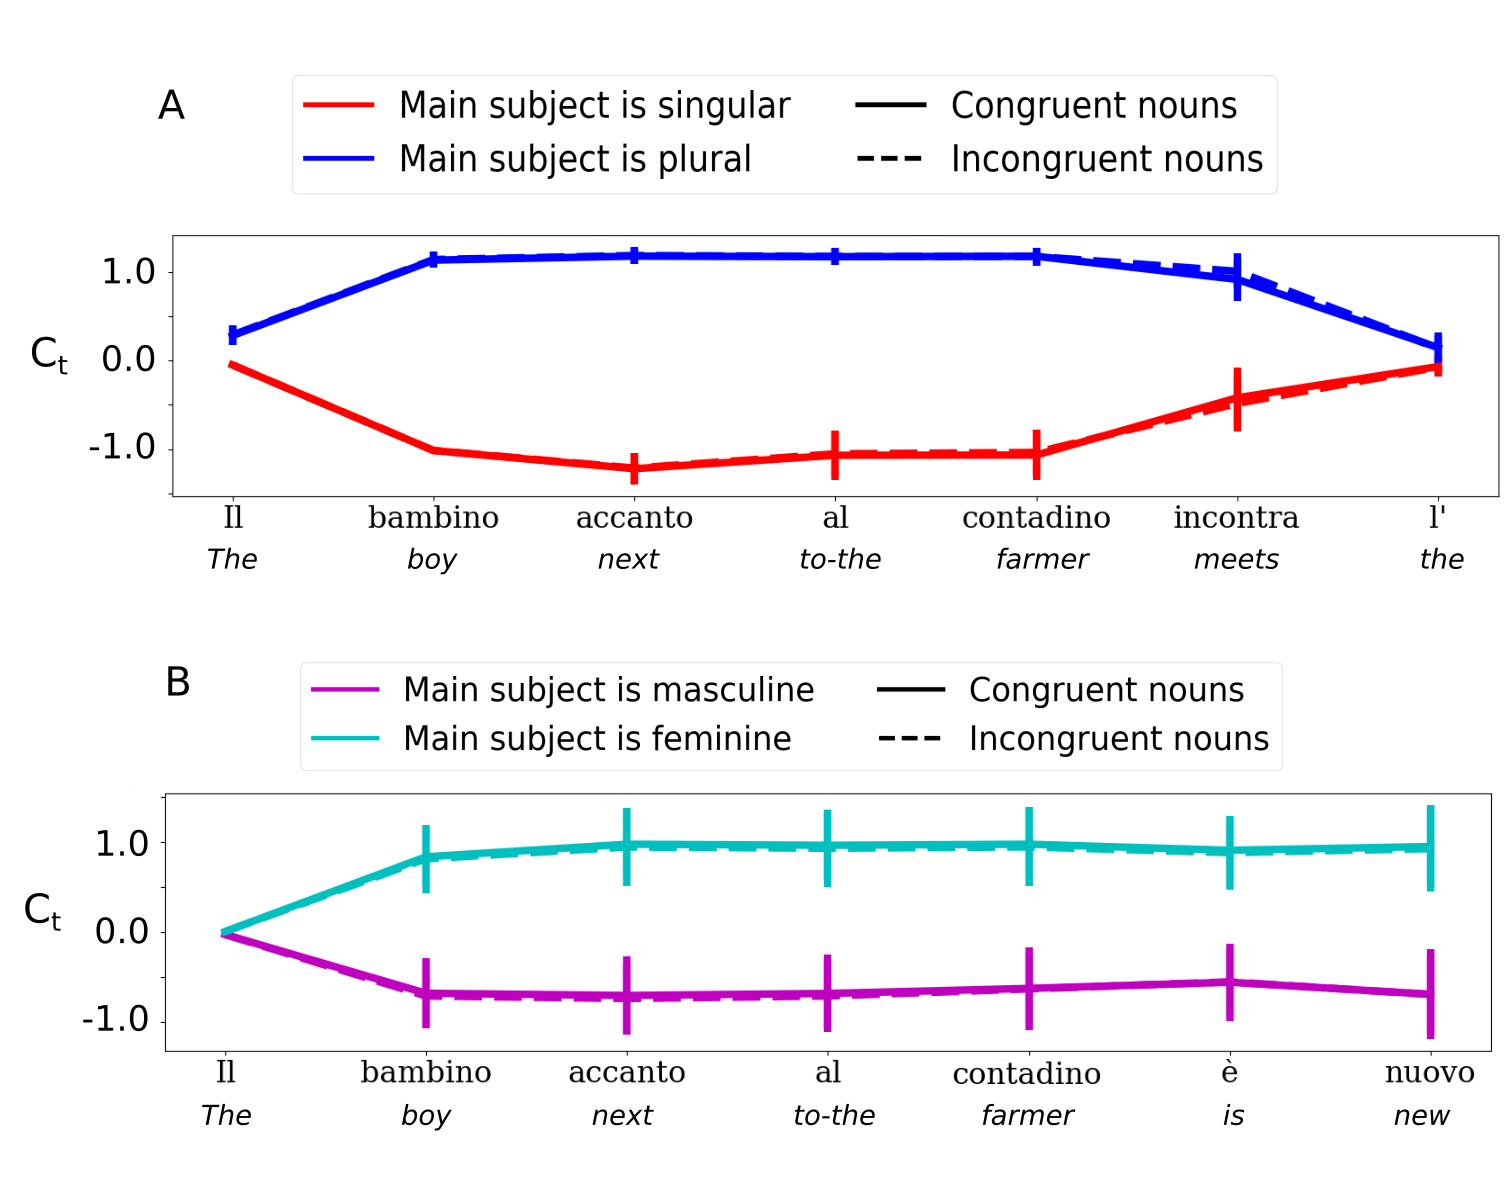
\includegraphics[width=\textwidth]{figures/model_activations_nounpp.png}
    \caption{\textbf{Cell activity of the number unit (panel A) and gender unit (panel B) during the processing of a single long-range dependency across a prepositional phrase:} four conditions are presented, corresponding to whether the main subject of the sentence is singular (red curves) or plural (blue), and to whether the main subject (`bambino') and the intervening noun (`contadino/figlio') have the same (congruent) or opposite number/gender (incongruent)}
    \label{fig:nounpp}
\end{figure} 

\subsubsection{Dynamics of the Number Unit Show Robustness to Attractors} 
To confirm that unit 815 is a long-range number unit, we visualize the dynamics of the unit during the processing of the long-range dependency, by extracting its activations during the processing of all sentences in the NounPP NA-task. Figure \ref{fig:nounpp}A describes the resulting average cell-state activations. It shows that number information is robustly encoded throughout the subject-verb dependency, also in the presence of an attractor (dashed lines). Furthermore, the dynamics of unit 815 show that it encodes both singular and plural number, using negative and positive cell activations, respectively. This is different from the English NLM, that developed two separate long-range units specialized on singular and plural respectively.

\subsubsection{Efferent Weights of the Number Unit are Clustered with Respect to Number}
Finally, we extract the efferent weights of unit 815, which project onto the output layer. Figure S2A shows that unit 815 differentially affects unit activations in the output layer, depending on whether they represent singular or plural forms of the verb. This is consistent with its role as a number unit. In what follows, we refer to unit 815 as the long-range `Number Unit'.

\subsubsection{Short-Range Number Units are also Found in the Network}
As was shown for the English NLM, long-range number units are not the only number-carrying units in the network. `Short-Range' number units also encode grammatical number. However, their activation is not robust to intervening numbers of local attractors. We therefore tested for the presence of short-range number units in the Italian NLM. We found 10 more number units, which encode grammatical number in separate values, and whose efferent weights are clustered with respect to number. \textbf{M: Should this point to a supplementary section?}

\subsubsection{Long-Range Gender Units are Also Found in the Network }
Agreement in Italian can also occur with respect to gender, for instance, in sentences containing predicative adjectives: ``\textbf{il bambino} accanto \emph{alla madre} \`{e} \textbf{bello}'' (``The (m.) boy near the (f.) mother is pretty (m.)''), in which subject and predicate agree with respect to both number and gender. We therefore hypothesize that there should also exist long-range `gender' units in the network, with dynamics that are robust to possible attractors (e.g., to ``madre'' above, which is feminine). 
To test this, we design a NA-task with adjective predicates and repeat the ablation study (Methods). 
We find one unit dramatically reducing the performance of the NLM when ablated. Its inner-state dynamics show robust encoding across the subject-adjective dependency (Figure \ref{fig:nounpp}B), also in the presence of attractors (dashed lines). Connectivity analysis further confirms that the efferent weights of the long-range `gender' unit are clustered with respect to whether they project to masculine or feminine adjective words in the output layer (figure S2B).



\vspace{10pt}
In sum, these results extend previous findings to another language and another grammatical feature. Similarly to English, only a few long-range number units emerged in the Italian NLMs during training. The NLM has developed a similar encoding scheme for both grammatical number and gender, independently. Taken together, this shows that sparse long-range feature units consistently emerge in NLMs.




